\iffalse

Nico Casale
Cody Orazymbetov

ECE 592 HW 3

\fi

\documentclass[]{../../ncmathy}

\begin{document}

A simple path is defined as \textbf{a path which contains no repeated vertices.} Both directed and undirected graphs can exist as fully connected graphs, where each vertex is connected to each other. i.e. there is a path from any vertex to another. Likewise, both directed and undirected graphs can be defined as multi-graphs, where multiple (redundant) edges can connect vertices. 
\\\\
If we have a graph $G(V,E)$ consisting of vertices $V$ and edges $E$, where a path exists between vertices $v_j$ and $v_k$, we can show that there exists a simple path that also connects the two vertices. 
\\\\
Assume that there only exists a path that contains repeated vertices between $v_j$ and $v_k$. The simple path is found as the first subset of the path that doesn't have repeated vertices. Take the following example:

\begin{figure}[H]
\centering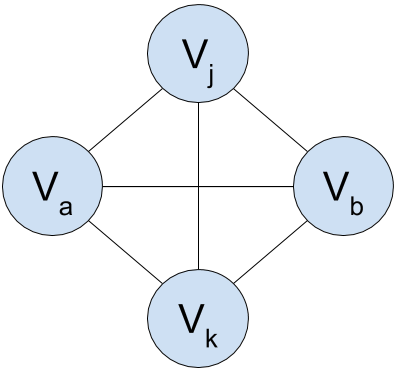
\includegraphics[width=0.4\textwidth]{exGraph}
\caption{A graph with cycles has at least one simple path between vertices $v_j$ and $v_k$.}
\end{figure}

The path between $v_j$ and $v_k$ can be represented in an infinite combination of ways, assuming vertices can be duplicated in a path. For instance, the path

\begin{equation}
	p_1 = (V_j, V_a, V_b, V_j, V_k)
\end{equation}

Reveals a simple path between $V_j$ and $V_k$ as simply the two nodes: $p_{simple} = (V_j, V_k)$. If there needed to be another connection through $V_b$ to reach $V_k$, the simple path would just have $V_b$ between the two nodes. As long as a path exists between $V_j$ and $V_k$, even one with duplicate nodes, a simple path can be extracted from it by virtue of its ultimate connection.

\end{document}